% This file was created with tikzplotlib v0.10.1.
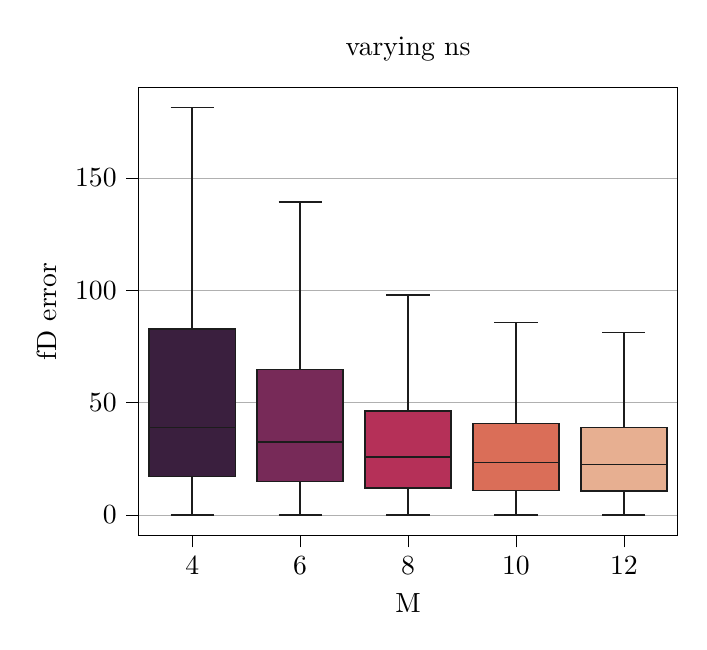
\begin{tikzpicture}

\definecolor{black28}{RGB}{28,28,28}
\definecolor{brown1814888}{RGB}{181,48,88}
\definecolor{burlywood231175145}{RGB}{231,175,145}
\definecolor{darkgray176}{RGB}{176,176,176}
\definecolor{darkslategray583162}{RGB}{58,31,62}
\definecolor{indianred21811088}{RGB}{218,110,88}
\definecolor{purple1194288}{RGB}{119,42,88}

\begin{axis}[
tick align=outside,
tick pos=left,
title={varying ns},
x grid style={darkgray176},
xlabel={M},
xmin=-0.5, xmax=4.5,
xtick style={color=black},
xtick={0,1,2,3,4},
xticklabels={4,6,8,10,12},
y grid style={darkgray176},
ylabel={fD error},
ymajorgrids,
ymin=-9.06968463878928, ymax=190.467045913826,
ytick style={color=black}
]
\path [draw=black28, fill=darkslategray583162, semithick]
(axis cs:-0.4,17.122973332579)
--(axis cs:0.4,17.122973332579)
--(axis cs:0.4,82.8990126457678)
--(axis cs:-0.4,82.8990126457678)
--(axis cs:-0.4,17.122973332579)
--cycle;
\path [draw=black28, fill=purple1194288, semithick]
(axis cs:0.6,14.9549997366975)
--(axis cs:1.4,14.9549997366975)
--(axis cs:1.4,64.7227914388888)
--(axis cs:0.6,64.7227914388888)
--(axis cs:0.6,14.9549997366975)
--cycle;
\path [draw=black28, fill=brown1814888, semithick]
(axis cs:1.6,12.0077412537376)
--(axis cs:2.4,12.0077412537376)
--(axis cs:2.4,46.432165428753)
--(axis cs:1.6,46.432165428753)
--(axis cs:1.6,12.0077412537376)
--cycle;
\path [draw=black28, fill=indianred21811088, semithick]
(axis cs:2.6,10.8762641799366)
--(axis cs:3.4,10.8762641799366)
--(axis cs:3.4,40.8309853125523)
--(axis cs:2.6,40.8309853125523)
--(axis cs:2.6,10.8762641799366)
--cycle;
\path [draw=black28, fill=burlywood231175145, semithick]
(axis cs:3.6,10.8241160515946)
--(axis cs:4.4,10.8241160515946)
--(axis cs:4.4,39.0229752717967)
--(axis cs:3.6,39.0229752717967)
--(axis cs:3.6,10.8241160515946)
--cycle;
\addplot [semithick, black28]
table {%
0 17.122973332579
0 0.000166749965956114
};
\addplot [semithick, black28]
table {%
0 82.8990126457678
0 181.397194525071
};
\addplot [semithick, black28]
table {%
-0.2 0.000166749965956114
0.2 0.000166749965956114
};
\addplot [semithick, black28]
table {%
-0.2 181.397194525071
0.2 181.397194525071
};
\addplot [semithick, black28]
table {%
1 14.9549997366975
1 0.00298682008030937
};
\addplot [semithick, black28]
table {%
1 64.7227914388888
1 139.259393463877
};
\addplot [semithick, black28]
table {%
0.8 0.00298682008030937
1.2 0.00298682008030937
};
\addplot [semithick, black28]
table {%
0.8 139.259393463877
1.2 139.259393463877
};
\addplot [semithick, black28]
table {%
2 12.0077412537376
2 0.00250963476685229
};
\addplot [semithick, black28]
table {%
2 46.432165428753
2 98.0564885447077
};
\addplot [semithick, black28]
table {%
1.8 0.00250963476685229
2.2 0.00250963476685229
};
\addplot [semithick, black28]
table {%
1.8 98.0564885447077
2.2 98.0564885447077
};
\addplot [semithick, black28]
table {%
3 10.8762641799366
3 0.0049743989777653
};
\addplot [semithick, black28]
table {%
3 40.8309853125523
3 85.6847433367634
};
\addplot [semithick, black28]
table {%
2.8 0.0049743989777653
3.2 0.0049743989777653
};
\addplot [semithick, black28]
table {%
2.8 85.6847433367634
3.2 85.6847433367634
};
\addplot [semithick, black28]
table {%
4 10.8241160515946
4 0.00131753468457418
};
\addplot [semithick, black28]
table {%
4 39.0229752717967
4 81.2772207388036
};
\addplot [semithick, black28]
table {%
3.8 0.00131753468457418
4.2 0.00131753468457418
};
\addplot [semithick, black28]
table {%
3.8 81.2772207388036
4.2 81.2772207388036
};
\addplot [semithick, black28]
table {%
-0.4 38.9676769062485
0.4 38.9676769062485
};
\addplot [semithick, black28]
table {%
0.6 32.5190613383658
1.4 32.5190613383658
};
\addplot [semithick, black28]
table {%
1.6 25.9573611128848
2.4 25.9573611128848
};
\addplot [semithick, black28]
table {%
2.6 23.3882302366415
3.4 23.3882302366415
};
\addplot [semithick, black28]
table {%
3.6 22.4975037611908
4.4 22.4975037611908
};
\end{axis}

\end{tikzpicture}
